\documentclass[11pt]{article}

% ------------------------------------------------------------
% Standard LaTeX packages
% ------------------------------------------------------------
\usepackage[margin=1in]{geometry}
\usepackage{amsmath,amssymb,mathtools}
\usepackage{amsthm}
\usepackage[american]{babel}
\usepackage{stmaryrd}
\usepackage{enumitem}
\usepackage{booktabs}
\usepackage{array}
\usepackage{listings}
\usepackage[x11names,table]{xcolor}
\usepackage{mdframed}
\usepackage{tikz}
\usetikzlibrary{arrows.meta,positioning,calc,decorations.pathmorphing}
\usepackage{url}
\usepackage[colorlinks=true,linkcolor=blue,citecolor=blue,urlcolor=blue]{hyperref}

% ---------- Cyrillic Sha Symbol ----------
\DeclareFontFamily{U}{wncy}{}
\DeclareFontShape{U}{wncy}{m}{n}{<->wncyr10}{}
\DeclareSymbolFont{mcy}{U}{wncy}{m}{n}
\DeclareMathSymbol{\Sha}{\mathord}{mcy}{"58}

% ---------- Theorem environments ----------
\theoremstyle{plain}
\newtheorem{theorem}{Theorem}[section]
\newtheorem{proposition}[theorem]{Proposition}
\newtheorem{lemma}[theorem]{Lemma}
\newtheorem{corollary}[theorem]{Corollary}
\newtheorem{conjecture}[theorem]{Conjecture}

\theoremstyle{definition}
\newtheorem{definition}[theorem]{Definition}
\newtheorem{axiombox}[theorem]{Axiom}
\newtheorem{protocol}[theorem]{Protocol}
\newtheorem{example}[theorem]{Example}

\theoremstyle{remark}
\newtheorem{remark}[theorem]{Remark}

% ---------- Notation ----------
\newcommand{\N}{\mathbb{N}}
\newcommand{\Z}{\mathbb{Z}}
\newcommand{\Q}{\mathbb{Q}}
\newcommand{\R}{\mathbb{R}}
\newcommand{\C}{\mathbb{C}}
\newcommand{\PP}{\mathbb{P}}
\newcommand{\F}{\mathbb{F}}
\newcommand{\calO}{\mathcal{O}}
\newcommand{\calL}{\mathcal{L}}
\newcommand{\Gal}{\mathrm{Gal}}
\newcommand{\GL}{\mathrm{GL}}
\newcommand{\SL}{\mathrm{SL}}
\newcommand{\Sel}{\mathrm{Sel}}
\usepackage{graphicx}
% Sha symbol declared above via wncyr10
\newcommand{\End}{\mathrm{End}}
\newcommand{\Frob}{\mathrm{Frob}}
\newcommand{\CRM}{\mathrm{CRM}}
\newcommand{\tr}{\mathrm{tr}}
\newcommand{\rk}{\mathrm{rk}}
\newcommand{\ord}{\mathrm{ord}}
\newcommand{\AJ}{\mathrm{AJ}}
\newcommand{\Reg}{\mathrm{Reg}}

\newcommand{\BISH}{\ensuremath{\mathsf{BISH}}}
\newcommand{\LPO}{\ensuremath{\mathsf{LPO}}}
\newcommand{\WLPO}{\ensuremath{\mathsf{WLPO}}}
\newcommand{\LLPO}{\ensuremath{\mathsf{LLPO}}}
\newcommand{\MP}{\ensuremath{\mathsf{MP}}}
\newcommand{\FT}{\ensuremath{\mathsf{FT}}}
\newcommand{\CLASS}{\ensuremath{\mathsf{CLASS}}}

\newcommand{\hhat}{\hat{h}}

% ---------- Code listing style for Lean ----------
\definecolor{codegreen}{rgb}{0,0.6,0}
\definecolor{codegray}{rgb}{0.5,0.5,0.5}
\definecolor{codepurple}{rgb}{0.58,0,0.82}
\definecolor{backcolour}{rgb}{0.95,0.95,0.92}

\lstdefinestyle{leanstyle}{
  backgroundcolor=\color{backcolour},
  commentstyle=\color{codegreen},
  keywordstyle=\color{blue},
  stringstyle=\color{codepurple},
  basicstyle=\ttfamily\footnotesize,
  breaklines=true,
  keepspaces=true,
  numbers=left,
  numberstyle=\tiny\color{codegray},
  showstringspaces=false,
  tabsize=2,
  frame=single,
  morekeywords={theorem,def,axiom,inductive,structure,where,instance,
    namespace,end,open,import,noncomputable,deriving,by,exact,intro,
    cases,constructor,rfl,rw,unfold,simp,decide,absurd,have,fun,let,
    show,with,Type,Prop,Sort},
  literate={ℚ}{{$\mathbb{Q}$}}1 {ℤ}{{$\mathbb{Z}$}}1 {ℕ}{{$\mathbb{N}$}}1 {ℝ}{{$\mathbb{R}$}}1 {≠}{{$\neq$}}1
}

% ---------- CRM box ----------
\newmdenv[
  linewidth=1pt,
  linecolor=blue!50!black,
  backgroundcolor=blue!3,
  roundcorner=3pt,
  innertopmargin=8pt,
  innerbottommargin=8pt
]{crmbox}

% ============================================================
\begin{document}

\title{The Root Number Bifurcation: CRM Cost of BSD Detection\\
Is Controlled by the Functional Equation\\[6pt]
\large Paper~96 of the Constructive Reverse Mathematics Series}

\author{Paul Chun-Kit Lee\\
\small New York University, Brooklyn, New York\\
\small \texttt{dr.paul.c.lee@gmail.com}}

\date{February 2026}

\maketitle

% ============================================================
\begin{abstract}
The CRM cost of detecting $L^{(r)}(E,1) \neq 0$ for the BSD conjecture is controlled by the root number $w = \pm 1$. For rank-0 curves ($w = +1$), modular symbols compute $L(E,1)/\Omega^+ \in \Q$, and non-vanishing is verified by \texttt{norm\_num}: detection is $\BISH$. For rank-1 curves ($w = -1$), the Gross--Zagier formula requires the Rankin--Selberg integral: detection is $\CLASS$. We prove four results using two test cases: $\texttt{11a1}$ ($y^2 + y = x^3 - x^2 - 10x - 20$, rank~0, $w = +1$) and $\texttt{37a1}$ ($y^2 + y = x^3 - x$, rank~1, $w = -1$). \textbf{Theorem~A}: the Hecke eigenvalue arithmetic and modular symbol $L(E,1)/\Omega^+ = 1/5 \neq 0$ for \texttt{11a1} are strictly $\BISH$ (27 sub-results, \texttt{native\_decide} and \texttt{norm\_num}). \textbf{Theorem~B}: the CRM cost of BSD detection bifurcates at $w = -1$: 10~$\BISH$ + 3~$\CLASS$ for rank~0 (77\%) versus 15~$\BISH$ + 6~$\CLASS$ for rank~1 (71\%). Existence is $\CLASS$ regardless of~$w$. \textbf{Theorem~C}: explicit 2-descent gives $\rk\, E(\Q) \leq 1$ for \texttt{37a1} without Kolyvagin---rank bounding is $\BISH$; $\Sha$ finiteness is irreducibly $\CLASS$. \textbf{Theorem~D}: across four Squeeze campaigns (Hodge P84--89, CY3 P94, BSD rank~1 P95, BSD rank~0 P96), existence is universally $\CLASS$; detection is $\BISH$ except when forced to $\CLASS$ by a computable invariant (root number, palindromic obstruction). Lean~4 verification: 1{,}033~lines, 86~theorems, 0~\texttt{sorry}.
\end{abstract}

% ============================================================
\section{Introduction}
\label{sec:intro}

\subsection{From rank 1 to rank 0}

Paper~95 \cite{paper95} applied the CRMLint Squeeze to the Gross--Zagier--Kolyvagin proof of BSD for analytic rank~$\leq 1$, using the rank-1 curve $\texttt{37a1}$ as test case. The decomposition was $15$~$\BISH$ + $6$~$\CLASS$ ($71\%$ constructive), with the $\CLASS$ content concentrated in the Rankin--Selberg integral and Kolyvagin's local duality. Detection of $L'(E,1) \neq 0$ required the Gross--Zagier formula ($\CLASS$).

Paper~96 asks: \emph{what happens at rank~0?} For elliptic curves with root number $w = +1$ (even functional equation), the order of vanishing $\ord_{s=1} L(E,s)$ is even, and if $L(E,1) \neq 0$, the BSD conjecture predicts rank~0. The key observation: for rank~0 curves, $L(E,1)/\Omega^+$ is a \emph{rational number}, computed by modular symbols as a finite sum involving Hecke eigenvalues \cite{cremona,manin}. Non-vanishing reduces to $1/5 \neq 0$---a \texttt{norm\_num} computation. No analytic continuation, no Rankin--Selberg, no Green's functions. Detection drops from $\CLASS$ to $\BISH$.

This is the BSD analogue of the palindromic bifurcation discovered in the Hodge campaign (Paper~89 \cite{paper89}): a computable invariant (the root number $w$ for BSD; the palindromic obstruction $a = c$ for Hodge) controls whether detection is $\BISH$ or $\CLASS$.

\subsection{The test cases}

\begin{itemize}[nosep]
\item \textbf{Rank 0:} $E = \texttt{11a1}$, given by $y^2 + y = x^3 - x^2 - 10x - 20$. Conductor $N = 11$, root number $w = +1$, torsion $E(\Q)_{\mathrm{tors}} \cong \Z/5\Z$, Tamagawa product $c_{11} = 5$ (Kodaira type $\mathrm{I}_5$), $|\Sha| = 1$, $L(E,1)/\Omega^+ = 1/5$.
\item \textbf{Rank 1:} $E = \texttt{37a1}$, given by $y^2 + y = x^3 - x$. Conductor $N = 37$, root number $w = -1$, trivial torsion, Tamagawa product $c_{37} = 1$, $|\Sha| = 1$, generator $(0,0)$.
\end{itemize}

Both are the simplest curves in their rank class: prime conductor, minimal discriminant, Cremona's first curves \cite{cremona,lmfdb}.

\subsection{Main results}

\begin{theorem}[Theorem A: Rank 0 Modular Symbol Core]
\label{thm:A}
For $E = \texttt{11a1}$, the Hecke eigenvalues $a_p$ for primes $p \leq 47$ satisfy: (i)~the point-count relation $a_p = p + 1 - \#E(\F_p)$ for 5 primes, (ii)~the Hecke recurrence $a_{p^2} = a_p^2 - p$ for 4 primes, (iii)~multiplicativity $a_{mn} = a_m a_n$ for 4 coprime pairs, and (iv)~the Hasse bound $a_p^2 \leq 4p$ for 14 primes. All 27 sub-results are verified by \texttt{native\_decide}. The modular symbol ratio $L(E,1)/\Omega^+ = 1/5 \neq 0$ is verified by \texttt{norm\_num}. Pure finite arithmetic: $\BISH$.
\end{theorem}

\begin{theorem}[Theorem B: Root Number Bifurcation]
\label{thm:B}
The CRM cost of BSD \emph{detection} (proving $L^{(r)}(E,1) \neq 0$) is controlled by the root number:
\begin{itemize}[nosep]
\item $w = +1$ (rank~0): detection is $\BISH$ (modular symbols compute $L(E,1)/\Omega^+ \in \Q$).
\item $w = -1$ (rank~1): detection is $\CLASS$ (Gross--Zagier formula requires Rankin--Selberg).
\end{itemize}
The CRM cost of BSD \emph{existence} (proving $\rk = r$ and $\Sha$ finite) is $\CLASS$ regardless of~$w$.

The component audit: $10$~$\BISH$ + $3$~$\CLASS = 13$ for rank~0 ($77\%$ constructive) versus $15$~$\BISH$ + $6$~$\CLASS = 21$ for rank~1 ($71\%$ constructive).
\end{theorem}

\begin{theorem}[Theorem C: Descent Excision]
\label{thm:C}
For $\texttt{37a1}$, explicit 2-descent gives $\rk\, E(\Q) \leq 1$ without Kolyvagin's Euler system. The 2-Selmer group has $\F_2$-rank~1 (CAS computation); since $E(\Q)[2] = 0$, we get $\rk\, E(\Q) \leq 1$. Combined with the generator $(0,0)$: $\rk\, E(\Q) = 1$. Rank bounding is $\BISH$ (descent is finite algebra); $\Sha$ finiteness is irreducibly $\CLASS$ (requires Euler system).
\end{theorem}

\begin{theorem}[Theorem D: Universal Detection/Existence Table]
\label{thm:D}
Across four Squeeze campaigns:
\begin{center}
\begin{tabular}{llll}
\toprule
\textbf{Papers} & \textbf{Domain} & \textbf{Detection} & \textbf{Existence} \\
\midrule
P84--89 & Hodge (Weil locus) & $\BISH$ & $\CLASS$ \\
P94 & CY3 (Griffiths group) & $\BISH$ & $\CLASS$ \\
P95 & BSD (rank 1, $w = -1$) & $\CLASS$ & $\CLASS$ \\
P96 & BSD (rank 0, $w = +1$) & $\BISH$ & $\CLASS$ \\
\bottomrule
\end{tabular}
\end{center}
Existence is universally $\CLASS$. Detection is $\BISH$ except when forced to $\CLASS$ by a computable invariant: the root number~$w$ for BSD, the palindromic obstruction for Hodge.
\end{theorem}

\subsection{Relationship to the series}

Paper~96 sits at the intersection of three threads:
\begin{itemize}[nosep]
\item The \emph{BSD thread} (Papers~48, 51, 95 \cite{paper48,paper51,paper95}): from diagnostic calibration of the conjecture to generative analysis of the proof, now extended to both rank classes.
\item The \emph{CRMLint Squeeze pipeline} (Papers~77--95 \cite{paper80,paper90}): Paper~96 is the fifteenth Squeeze application.
\item The \emph{bifurcation pattern} (Paper~89 \cite{paper89}): a computable invariant controls the $\BISH/\CLASS$ split of detection. The palindromic obstruction in the Hodge campaign finds its BSD analogue in the root number.
\end{itemize}

The connection between the palindromic bifurcation and the root number bifurcation is structural. In both cases, a \emph{symmetry} of the arithmetic object (palindromic symmetry of the characteristic polynomial; functional equation symmetry of $L(E,s)$) controls whether the algebraic shadow (trace identity; modular symbol) is sufficient for detection ($\BISH$) or whether a transcendental computation (Hodge conjecture; Gross--Zagier formula) is required ($\CLASS$).


% ============================================================
\section{Preliminaries}
\label{sec:prelim}

\subsection{CRM hierarchy}

The constructive reverse mathematics hierarchy \cite{bridges-richman,paper1,paper40}:
\[
\BISH \;\subsetneq\; \BISH{+}\MP \;\subsetneq\; \BISH{+}\LLPO \;\subsetneq\; \BISH{+}\WLPO \;\subsetneq\; \BISH{+}\LPO \;\subsetneq\; \CLASS.
\]
We refer to Papers~1--5 for definitions. The principles relevant here: $\BISH$ (bounded search, explicit witnesses), $\LPO$ (for real-number zero-testing), and $\CLASS$ (full classical logic).

\subsection{Modular symbols}

Let $f \in S_2(\Gamma_0(N))$ be the newform associated to an elliptic curve $E/\Q$ of conductor~$N$. The \emph{modular symbol} $[r \to s]^+ = \mathrm{Re}\int_r^s f(\tau)\,d\tau$ for $r, s \in \Q \cup \{\infty\}$ is a period integral computed by the Manin--Drinfeld theorem \cite{manin} as a finite rational linear combination. The ratio
\[
[0 \to \infty]^+ = \frac{L(E,1)}{\Omega^+}
\]
is a \emph{rational number}, computable from the Hecke eigenvalues by continued fraction expansion and Hecke action \cite{cremona}. For rank-0 curves ($L(E,1) \neq 0$), this ratio is nonzero. For rank-1 curves ($L(E,1) = 0$ by the functional equation), the ratio vanishes, and one must compute $L'(E,1)$ via the Gross--Zagier formula---an analytic computation.

\subsection{Root number and the functional equation}

The completed $L$-function $\Lambda(E,s) = N^{s/2}(2\pi)^{-s}\Gamma(s)L(E,s)$ satisfies
\[
\Lambda(E, s) = w \cdot \Lambda(E, 2-s)
\]
where $w = \pm 1$ is the \emph{root number}. At $s = 1$: $\Lambda(E,1) = w \cdot \Lambda(E,1)$, so $w = -1$ forces $L(E,1) = 0$. The root number is computable from local data (conductor exponents, reduction types) as a finite product of local root numbers: $\BISH$ \cite{silverman-aec}.

\subsection{Kato's Euler system for rank 0}

For rank-0 curves, Kato's Euler system \cite{kato} replaces Kolyvagin: if $L(E,1) \neq 0$, then $\rk\, E(\Q) = 0$ and $\Sha(E/\Q)$ is finite. The proof uses Beilinson elements, completed cohomology, and $p$-adic $L$-functions---all $\CLASS$. The key difference from rank~1: no Heegner point is needed, and the non-vanishing detection $L(E,1)/\Omega^+ \neq 0$ is a rational computation.

\subsection{2-descent}

The 2-descent computes the 2-Selmer group $\Sel^2(E/\Q)$, giving an upper bound $\rk\, E(\Q) \leq \dim_{\F_2} \Sel^2(E/\Q) - \dim_{\F_2} E(\Q)[2]$. This is a finite algebraic computation: factor the 2-division polynomial, compute local images, assemble via the Selmer exact sequence \cite{silverman-aec,cassels-descent}. The computation is $\BISH$: it involves finitely many local solubility checks over $\Q_p$ for finitely many primes~$p$.


% ============================================================
\section{The Modular Symbol Core (Theorem~A)}
\label{sec:hecke}

\subsection{Hecke eigenvalue table for 11a1}

The newform $f \in S_2(\Gamma_0(11))$ associated to $\texttt{11a1}$ has integral Hecke eigenvalues \cite{cremona}. Table~\ref{tab:hecke11a1} lists $a_p$ for primes $p \leq 47$, together with the point count $\#E(\F_p)$ and the Hasse bound check.

\begin{table}[ht]
\centering
\caption{Hecke eigenvalues for $\texttt{11a1}$: $y^2 + y = x^3 - x^2 - 10x - 20$.}\label{tab:hecke11a1}
\begin{tabular}{c r r c c}
\toprule
$p$ & $a_p$ & $\#E(\F_p)$ & $a_p = p+1-\#E$? & $a_p^2 \leq 4p$? \\
\midrule
2  & $-2$ & 5  & \checkmark & $4 \leq 8$ \\
3  & $-1$ & 5  & \checkmark & $1 \leq 12$ \\
5  & $1$  & 5  & \checkmark & $1 \leq 20$ \\
7  & $-2$ & 10 & \checkmark & $4 \leq 28$ \\
11 & $1$  & --- & (bad, $\mathrm{I}_5$) & --- \\
13 & $4$  & 10 & \checkmark & $16 \leq 52$ \\
17 & $-2$ & --- & --- & $4 \leq 68$ \\
19 & $0$  & --- & --- & $0 \leq 76$ \\
23 & $-1$ & --- & --- & $1 \leq 92$ \\
29 & $0$  & --- & --- & $0 \leq 116$ \\
31 & $7$  & --- & --- & $49 \leq 124$ \\
37 & $3$  & --- & --- & $9 \leq 148$ \\
41 & $-8$ & --- & --- & $64 \leq 164$ \\
43 & $-6$ & --- & --- & $36 \leq 172$ \\
47 & $8$  & --- & --- & $64 \leq 188$ \\
\bottomrule
\end{tabular}
\end{table}

\subsection{Point-count verification}

\begin{proposition}\label{prop:pointcount11a1}
For $E = \texttt{11a1}$: $y^2 + y = x^3 - x^2 - 10x - 20$ over $\F_p$, the point counts are as given in Table~\ref{tab:hecke11a1}.
\end{proposition}

\begin{proof}
We demonstrate the enumeration for $p = 2$ and $p = 5$.

\emph{Case $p = 2$.} Over $\F_2$, the equation reduces to $y^2 + y = x^3 + x^2$. For each $x \in \F_2$:
\begin{center}
\begin{tabular}{cccc}
$x$ & $x^3 + x^2 \pmod{2}$ & Solutions to $y^2 + y = r$ & Count \\
\hline
$0$ & $0$ & $y \in \{0, 1\}$ & 2 \\
$1$ & $0$ & $y \in \{0, 1\}$ & 2
\end{tabular}
\end{center}
Affine points: 4. Adding the point at infinity: $\#E(\F_2) = 5$. Hence $a_2 = 2 + 1 - 5 = -2$. \checkmark

\emph{Case $p = 5$.} Over $\F_5$, the equation is $y^2 + y = x^3 - x^2$ (since $-10x \equiv 0$ and $-20 \equiv 0 \pmod{5}$). The right-hand side for $x = 0, 1, 2, 3, 4$ gives $0, 0, 4, 3, 3 \pmod{5}$. The equation $y^2 + y = r$ in $\F_5$ has solutions for $r \in \{0, 1, 2\}$ with counts $2, 1, 2$, and no solutions for $r \in \{3, 4\}$. Counting the matches: $2 + 2 + 0 + 0 + 0 = 4$ affine points. Adding infinity: $\#E(\F_5) = 5$. Hence $a_5 = 5 + 1 - 5 = 1$. \checkmark

The remaining primes ($p = 3, 7, 13$) follow by the same exhaustive enumeration. In Lean, the entire table is checked by \texttt{native\_decide}.
\end{proof}

\subsection{Hecke recurrence and multiplicativity}

\begin{proposition}\label{prop:recurrence11a1}
For $\texttt{11a1}$, the Hecke eigenvalues satisfy:
\begin{enumerate}[nosep,label=(\roman*)]
\item $a_4 = a_2^2 - 2 = 4 - 2 = 2$, \quad $a_9 = a_3^2 - 3 = 1 - 3 = -2$,
\item $a_{25} = a_5^2 - 5 = 1 - 5 = -4$, \quad $a_{49} = a_7^2 - 7 = 4 - 7 = -3$.
\item $a_6 = a_2 \cdot a_3 = 2$, \quad $a_{10} = a_2 \cdot a_5 = -2$,
\item $a_{15} = a_3 \cdot a_5 = -1$, \quad $a_{35} = a_5 \cdot a_7 = -2$.
\end{enumerate}
All verified by \texttt{native\_decide} on the defined \texttt{hecke\_11a1} function.
\end{proposition}

\subsection{The modular symbol ratio}

\begin{proposition}\label{prop:modsym}
For $\texttt{11a1}$, the modular symbol ratio
\[
[0 \to \infty]^+ = \frac{L(E,1)}{\Omega^+} = \frac{1}{5}
\]
is computed by Cremona's algorithm \cite{cremona} (equivalently, \texttt{EllipticCurve('11a1').modular\_symbol()(0)} in Sage). Non-vanishing: $1/5 \neq 0$.
\end{proposition}

\begin{proof}
The modular symbol $[0 \to \infty]^+$ for $\Gamma_0(11)$ is computed by the Manin continued-fraction algorithm \cite{cremona}: one expands $0/1$ as a continued fraction, applies the Hecke operators $T_p$ to the path from $0$ to $i\infty$ in the upper half-plane, and accumulates the result as a $\Z$-linear combination of unimodular symbols $\{r, s\}$ for $r, s \in \Q$. For the unique newform in $S_2(\Gamma_0(11))$, this yields
\[
[0 \to \infty]^+ = \frac{L(E,1)}{\Omega^+} = \frac{1}{5}.
\]
The computation is purely algebraic: it uses only the Hecke eigenvalues $a_n \in \Z$ and the Manin relations (finitely many linear equations over $\Z$). The CAS (Sage, \texttt{EllipticCurve('11a1').modular\_symbol()(0)}) confirms $1/5$. Non-vanishing: $1/5 \neq 0$ is immediate. In Lean:
\begin{lstlisting}[style=leanstyle]
def modular_symbol_ratio_11a1 : Rat := 1 / 5
theorem modular_symbol_nonzero_11a1 :
    modular_symbol_ratio_11a1 ≠ 0 := by
  unfold modular_symbol_ratio_11a1; norm_num
\end{lstlisting}
The proof requires only \texttt{norm\_num}: rational arithmetic. No analytic continuation, no $\Gamma$-function, no integration. $\BISH$.
\end{proof}

\begin{remark}\label{rem:detection-contrast}
For $\texttt{37a1}$ (rank~1, $w = -1$), the modular symbol $[0 \to \infty]^+ = L(E,1)/\Omega^+ = 0$---the functional equation forces vanishing. Detecting $L'(E,1) \neq 0$ requires the Gross--Zagier formula \cite{gross-zagier}, which computes $L'(E,1)$ via the Rankin--Selberg convolution ($\CLASS$). The root number controls which detection mechanism is available.
\end{remark}


% ============================================================
\section{The BSD Formula for Rank 0 (Theorem~A continued)}
\label{sec:bsd-rank0}

\subsection{Arithmetic invariants of 11a1}

\begin{proposition}\label{prop:bsd-data}
For $E = \texttt{11a1}$:
\begin{enumerate}[nosep,label=(\roman*)]
\item $E(\Q)_{\mathrm{tors}} \cong \Z/5\Z$, $|E(\Q)_{\mathrm{tors}}| = 5$.
\item Tamagawa product: $\prod c_p = c_{11} = 5$ (Kodaira type $\mathrm{I}_5$ at $p = 11$, split multiplicative reduction since $a_{11} = 1$).
\item $|\Sha(E/\Q)| = 1$ (trivial).
\item $\rk\, E(\Q) = 0$ (confirmed by $L(E,1)/\Omega^+ = 1/5 \neq 0$ and Kato's theorem).
\end{enumerate}
Source: LMFDB \cite{lmfdb}, Cremona \cite{cremona}.
\end{proposition}

\subsection{BSD formula check}

The rank-0 BSD formula:
\begin{equation}\label{eq:bsd0}
\frac{L(E,1)}{\Omega^+} = |\Sha| \cdot \frac{\prod c_p}{|E(\Q)_{\mathrm{tors}}|^2}.
\end{equation}

\begin{proposition}\label{prop:bsd-check}
For $\texttt{11a1}$:
\[
\frac{1}{5} = 1 \cdot \frac{5}{25} = \frac{5}{25} = \frac{1}{5}. \quad \checkmark
\]
\end{proposition}

\begin{proof}
Substituting the arithmetic invariants from Proposition~\ref{prop:bsd-data} into the rank-0 BSD formula~\eqref{eq:bsd0}:
\[
\text{RHS} = |\Sha| \cdot \frac{\prod c_p}{|E(\Q)_{\mathrm{tors}}|^2}
= 1 \cdot \frac{5}{5^2}
= \frac{5}{25}
= \frac{1}{5}
= \frac{L(E,1)}{\Omega^+} = \text{LHS.}
\]
Each step is rational arithmetic: substitution of integers, multiplication, and cancellation. No real analysis, no limits, no approximation. In Lean, this is a single \texttt{norm\_num} invocation on the unfolded rational expressions:
\begin{lstlisting}[style=leanstyle]
theorem bsd_formula_matches_modular_symbol :
    modular_symbol_ratio_11a1 =
      (sha_order_11a1 : Rat) * tamagawa_product_11a1 /
      (torsion_order_11a1 * torsion_order_11a1) := by
  unfold modular_symbol_ratio_11a1 sha_order_11a1
    tamagawa_product_11a1 torsion_order_11a1; norm_num
\end{lstlisting}
The CRM classification: $\BISH$. The BSD formula check is pure rational arithmetic, contingent only on the correctness of the input data (torsion, Tamagawa, $\Sha$ order). The input data itself is $\BISH$: torsion is computed by the Nagell--Lutz theorem (finite search), Tamagawa numbers by Tate's algorithm (finitely many local computations), and $|\Sha| = 1$ is confirmed by the BSD formula consistency (given the other invariants and the modular symbol).
\end{proof}


% ============================================================
\section{The Root Number Bifurcation (Theorem~B)}
\label{sec:bifurcation}

\subsection{Detection at rank 0 versus rank 1}

The key structural difference:

\begin{crmbox}
\textbf{Rank 0 ($w = +1$):} $L(E,1)/\Omega^+$ is a nonzero rational number. Detection of $L(E,1) \neq 0$ is equivalent to $1/5 \neq 0$: \texttt{norm\_num}. $\BISH$.

\textbf{Rank 1 ($w = -1$):} $L(E,1) = 0$ (forced by the functional equation). Detection of $L'(E,1) \neq 0$ requires the Gross--Zagier formula, which computes $L'(E,1) = c_{\mathrm{GZ}} \cdot \hhat(y_K)$ via the Rankin--Selberg integral. $\CLASS$.
\end{crmbox}

\subsection{Component audits}

\begin{proof}[Proof of Theorem~B]
The argument has two parts: the \emph{mathematical} reason why the root number controls the CRM cost, and the \emph{component audit} that quantifies it.

\emph{Part 1: Why the root number controls detection cost.}
The modular symbol $[0 \to \infty]^+ = L(E,1)/\Omega^+$ is a rational number because it is computed by the Manin--Drinfeld theorem as a finite $\Z$-linear combination of Hecke operators applied to the winding element \cite{manin,cremona}. The computation requires only the $q$-expansion coefficients of the newform $f$, which are the Hecke eigenvalues $a_n$---integers computable by point counting over finite fields. No integration, no analytic continuation, no convergence argument: the modular symbol is a \emph{finite algebraic} object. Its non-vanishing is therefore a question of rational arithmetic ($\BISH$).

When $w = +1$, the functional equation implies $\ord_{s=1} L(E,s)$ is even. If $L(E,1) \neq 0$ (which the modular symbol test detects), then $\ord_{s=1} = 0$. The entire detection argument stays within $\BISH$.

When $w = -1$, the functional equation forces $L(E,1) = 0$, so $[0 \to \infty]^+ = 0$ identically. To detect $L'(E,1) \neq 0$, one must invoke the Gross--Zagier formula \cite{gross-zagier}:
\[
L'(E,1) = c_{\mathrm{GZ}} \cdot \hhat(y_K)
\]
where $y_K$ is the Heegner point and $c_{\mathrm{GZ}}$ involves the Petersson norm of $f$ and local factors. The Petersson norm $\langle f, f \rangle = \int_{\Gamma_0(N) \backslash \mathcal{H}} |f(\tau)|^2 \, d\mu$ is a non-compact integral over the modular curve --- an intrinsically analytic computation. The Rankin--Selberg method that relates this to $L'(E,1)$ requires the meromorphic continuation of the Rankin--Selberg convolution $L(f \times \overline{f}, s)$ to $s = 1$. Both are $\CLASS$.

Thus the root number $w$ determines which \emph{mathematical mechanism} is available for detection: rational modular symbols ($\BISH$) when $w = +1$, or the Gross--Zagier integral ($\CLASS$) when $w = -1$.

\emph{Part 2: Component audits.}

\emph{Rank 0 (11a1):} The proof that $\rk\, E(\Q) = 0$ and $\Sha$ is finite proceeds in two stages: (1)~compute the modular symbol $L(E,1)/\Omega^+ = 1/5 \neq 0$ ($\BISH$); (2)~invoke Kato's Euler system: $L(E,1) \neq 0 \Rightarrow \rk = 0$ and $|\Sha| < \infty$ ($\CLASS$). The $\BISH$ core comprises: Hecke eigenvalue table, point count verification, Hecke recurrence, Hecke multiplicativity, Hasse bounds, modular symbol ratio, modular symbol nonzero, torsion order, Tamagawa product, BSD formula check. The $\CLASS$ shell: analytic continuation, Kato Euler system, $\Sha$ finiteness. Total: $10$~$\BISH$ + $3$~$\CLASS = 13$ ($77\%$).

\emph{Rank 1 (37a1):} From Paper~95 \cite{paper95}: $15$~$\BISH$ + $6$~$\CLASS = 21$ ($71\%$). The additional $\CLASS$ components versus rank~0: Rankin--Selberg (Gross--Zagier), archimedean local heights, Cassels pairing, Poitou--Tate, Chebotarev density. These are all absent from the rank-0 pipeline because rank-0 detection requires no Heegner point, no height computation, and no local duality.

The detection bifurcation: detection is $\BISH$ for rank~0, $\CLASS$ for rank~1. Existence ($\rk = r$, $\Sha$ finite) is $\CLASS$ for both. In Lean:
\begin{lstlisting}[style=leanstyle]
theorem detection_bifurcation :
    rank0_bifurcation.detection_level = BISH /\
    rank1_bifurcation.detection_level = CLASS := by
  constructor <;> rfl
\end{lstlisting}
This theorem has \emph{zero axioms}: the detection levels are definitional, and the proof is by \texttt{rfl} on both conjuncts.
\end{proof}

\subsection{The BISH fraction improves}

The rank-0 audit achieves $77\%$ $\BISH$ versus $71\%$ for rank~1. The improvement is structural: rank~0 eliminates the Gross--Zagier formula (the main source of $\CLASS$ content in rank~1) and replaces it with the modular symbol computation (which is $\BISH$). The only $\CLASS$ ingredients for rank~0 are Kato's Euler system and $\Sha$ finiteness---the \emph{existence} side.

\begin{proposition}\label{prop:fraction}
$10/13 > 15/21$, i.e., the rank-0 BISH fraction strictly exceeds the rank-1 fraction.
\end{proposition}

\begin{proof}
$10 \times 21 = 210 > 195 = 15 \times 13$. Verified by \texttt{native\_decide}.
\end{proof}


% ============================================================
\section{Descent Excision (Theorem~C)}
\label{sec:descent}

\subsection{2-descent for 37a1}

The 2-descent computes $\dim_{\F_2} \Sel^2(E/\Q)$ for $E = \texttt{37a1}$.

\begin{proposition}\label{prop:selmer}
$\dim_{\F_2} \Sel^2(\texttt{37a1}/\Q) = 1$ and $E(\Q)[2] = 0$.
\end{proposition}

\begin{proof}
The 2-Selmer rank is computed by Sage (\texttt{EllipticCurve('37a1').selmer\_rank()}) or equivalently by Cremona's \texttt{mwrank} \cite{cremona}. The curve $y^2 + y = x^3 - x$ transforms via $y \mapsto y - 1/2$ into $(2y)^2 = 4x^3 - 4x + 1$. The $2$-division polynomial $4x^3 - 4x + 1$ has discriminant $592 > 0$ and three real roots, but by the Rational Root Theorem its only possible rational roots are $\pm 1, \pm 1/2, \pm 1/4$, none of which evaluate to zero. Thus it is irreducible over~$\Q$, and $E(\Q)[2] = 0$.

From the exact sequence $0 \to E(\Q)/2E(\Q) \to \Sel^2(E/\Q) \to \Sha(E/\Q)[2] \to 0$, we get $\rk\, E(\Q) \leq \dim_{\F_2} \Sel^2 - \dim_{\F_2} E(\Q)[2] = 1 - 0 = 1$.
\end{proof}

\begin{proof}[Proof of Theorem~C]
The 2-descent gives $\rk\, E(\Q) \leq 1$ without invoking Kolyvagin. Combined with the known point $(0,0) \in E(\Q)$ of infinite order (verified: the curve equation $0^2 + 0 = 0^3 - 0$ holds, and $\hhat(0,0) > 0$ from Paper~95), we get $\rk\, E(\Q) = 1$.

The meta-theorem:
\begin{itemize}[nosep]
\item \textbf{Rank bounding} ($\rk \leq 1$): $\BISH$. The 2-descent is finite algebra over $\Q$ and $\Q_p$ for finitely many~$p$. No analytic input.
\item \textbf{$\Sha$ finiteness}: irreducibly $\CLASS$. Descent gives $\dim \Sha[2] \leq \dim \Sel^2 - \rk = 0$, but finiteness of the full $\Sha$ (not just the 2-part) requires Kolyvagin's Euler system.
\end{itemize}

In Lean, this is formalized via the \texttt{KolyvaginExcision} structure:
\begin{lstlisting}[style=leanstyle]
structure KolyvaginExcision where
  rank_bound_level : CRMLevel
  sha_finite_level : CRMLevel

def kolyvagin_excision_37a1 : KolyvaginExcision := {
  rank_bound_level := BISH,
  sha_finite_level := CLASS
}

theorem descent_excises_rank :
    kolyvagin_excision_37a1.rank_bound_level = BISH := rfl
\end{lstlisting}
\end{proof}


% ============================================================
\section{Universal Detection/Existence Table (Theorem~D)}
\label{sec:universal}

\subsection{The four campaigns}

\begin{proof}[Proof of Theorem~D]
We compile the bifurcation landscape across all CRMLint Squeeze campaigns and argue for the universality of each pattern.

\begin{center}
\begin{tabular}{lllll}
\toprule
\textbf{Papers} & \textbf{Domain} & \textbf{Detection} & \textbf{Existence} & \textbf{Control} \\
\midrule
P84--89 & Hodge (Weil locus) & $\BISH$ & $\CLASS$ & palindromic $(a = c)$ \\
P94 & CY3 (Griffiths) & $\BISH$ & $\CLASS$ & source $\delta(z)$ \\
P95 & BSD ($w = -1$) & $\CLASS$ & $\CLASS$ & root number $w$ \\
P96 & BSD ($w = +1$) & $\BISH$ & $\CLASS$ & root number $w$ \\
\bottomrule
\end{tabular}
\end{center}

\textbf{Existence is universally $\CLASS$.} We argue case by case that this is not accidental but structural.

\emph{Hodge (P84--89):} Proving that a cohomology class is algebraic requires Weyl's theorem on invariants of compact Lie groups (algebraicity of $\mathrm{GSp}_4$-invariant classes). The compactness of $\mathrm{GSp}_4(\R)$ is a topological input; the representation-theoretic classification uses the existence of Haar measure. Both are $\CLASS$.

\emph{CY3 (P94):} Proving that the Griffiths group $\mathrm{Griff}^2(X)$ is infinite (contains a non-torsion element) requires the Abel--Jacobi map $\Phi: \mathrm{CH}^2(X)_{\mathrm{hom}} \to J^2(X)$ and the Baire category theorem to establish injectivity on a dense subset. The Baire argument is $\CLASS$.

\emph{BSD rank~1 (P95):} Proving $\rk\, E(\Q) = 1$ and $\Sha$ finite requires Kolyvagin's Euler system. The key step is the annihilation of $\Sha$ by derivative classes $\kappa_n$, constructed from Heegner points via local duality (Poitou--Tate). The local duality sequence involves completion at all places of $\Q$ and a product over infinitely many primes, which is $\CLASS$.

\emph{BSD rank~0 (P96):} Proving $\rk\, E(\Q) = 0$ and $\Sha$ finite requires Kato's Euler system. The key step is bounding the Selmer group via Beilinson elements in $K_2$ of modular curves and the main conjecture of Iwasawa theory. The $p$-adic $L$-function is constructed as a $p$-adic measure (a limit in the Iwasawa algebra), which is $\CLASS$.

In each case, the existence proof requires passing from a \emph{local} or \emph{finite} algebraic computation to a \emph{global} structural conclusion (finiteness, algebraicity, rank bound). The passage involves either: a compactness argument, a limit in a complete topological ring, or an infinite product over all places. These are the hallmarks of $\CLASS$.

In Lean, the universality is verified by:
\begin{lstlisting}[style=leanstyle]
theorem existence_universally_class :
    forall s in squeeze_landscape, s.existence = CLASS := by
  simp [squeeze_landscape]
\end{lstlisting}

\textbf{Detection is mostly $\BISH$.} In 3 of 4 campaigns, detecting that an arithmetic object is non-trivial reduces to a finite algebraic computation: trace identity ($\tau_+ = 0$ by \texttt{ring} on polynomial coefficients), algebraic source term ($\delta(z) \neq 0$ by \texttt{ring}), modular symbol ($L(E,1)/\Omega^+ = 1/5 \neq 0$ by \texttt{norm\_num}). Each detection proof terminates in finitely many steps with an explicit witness or certificate.

The single exception is rank-1 BSD, where detection requires the Gross--Zagier formula ($\CLASS$). The exception is forced by the root number $w = -1$: the functional equation zeroes out $L(E,1)$, making the zero-order algebraic shadow trivially zero. The first non-vanishing derivative $L'(E,1)$ can only be accessed through the Rankin--Selberg integral, which is a non-compact analytic computation.

The pattern: detection produces a \emph{finite algebraic certificate} (a rational number, a polynomial identity, a trace value) that can be checked by a terminating computation. Existence requires a \emph{global structural argument} (an Euler system, a compactness theorem, a Baire category argument) that involves infinitary reasoning.
\end{proof}

\subsection{The structural pattern}

The universal pattern: the \emph{algebraic shadow} of a transcendental object is constructively accessible, while the transcendental object itself requires classical principles.

\begin{center}
\begin{tabular}{lll}
\toprule
\textbf{Transcendental object} & \textbf{Algebraic shadow} & \textbf{Shadow status} \\
\midrule
$L'(E,1)$ (analytic) & $L(E,1)/\Omega^+ \in \Q$ (modular symbol) & $\BISH$ (if $w = +1$) \\
Hodge class (topology) & $\tau_+ = 0$ (trace identity) & $\BISH$ (if palindromic) \\
Normal function (analysis) & $\delta(z)$ (algebraic source) & $\BISH$ \\
$L'(E,1)$ (odd rank) & $\hhat(y_K) > 0$ (Gross--Zagier) & $\CLASS$ \\
\bottomrule
\end{tabular}
\end{center}

The root number controls whether the algebraic shadow is sufficient. When $w = +1$, the zero-order shadow $L(E,1)/\Omega^+$ is nonzero and computable. When $w = -1$, the zero-order shadow vanishes, and one must access the first derivative $L'(E,1)$ through a transcendental formula.


% ============================================================
\section{CRM Audit}
\label{sec:audit}

\subsection{Classification}

\begin{center}
\begin{tabular}{lll}
\toprule
\textbf{Component} & \textbf{CRM Level} & \textbf{Justification} \\
\midrule
\multicolumn{3}{l}{\emph{Rank 0 (11a1) --- 10 $\BISH$ + 3 $\CLASS$}} \\
Hecke eigenvalue table & $\BISH$ & Verified by enumeration \\
Point count verification & $\BISH$ & Exhaustive enumeration over $\F_p$ \\
Hecke recurrence & $\BISH$ & Arithmetic identities \\
Hecke multiplicativity & $\BISH$ & Arithmetic identities \\
Hasse bound & $\BISH$ & Integer inequality \\
Modular symbol ratio $= 1/5$ & $\BISH$ & Rational computation (Cremona) \\
Modular symbol ratio $\neq 0$ & $\BISH$ & $1/5 \neq 0$: \texttt{norm\_num} \\
Torsion order $= 5$ & $\BISH$ & Finite computation (Tate alg.)\ \\
Tamagawa product $= 5$ & $\BISH$ & Finite computation \\
BSD formula check & $\BISH$ & $1/5 = 1 \cdot 5/25$: \texttt{norm\_num} \\
\midrule
Analytic continuation & $\CLASS$ & Mellin transform, $\Gamma$-function \\
Kato Euler system & $\CLASS$ & Beilinson elements, $p$-adic $L$ \\
$\Sha$ finiteness & $\CLASS$ & Requires Euler system \\
\midrule
\multicolumn{3}{l}{\emph{Rank 1 (37a1) --- from Paper~95: 15 $\BISH$ + 6 $\CLASS$}} \\
\bottomrule
\end{tabular}
\end{center}

\subsection{What descends}

\begin{itemize}[nosep]
\item \textbf{L-value detection:} from $\CLASS$ to $\BISH$ (at rank~0). The modular symbol computes $L(E,1)/\Omega^+ \in \Q$ without analytic continuation.
\item \textbf{Rank bounding:} from $\CLASS$ (Kolyvagin) to $\BISH$ (2-descent). Explicit descent excises the Euler system from the rank bound.
\item \textbf{$\Sha$ finiteness:} does \emph{not} descend. Irreducibly $\CLASS$ at both ranks. This is the Classical Boundary Node for the existence side.
\end{itemize}

\subsection{Classical Boundary Nodes}

For rank~0, the irreducible $\CLASS$ content is Kato's Euler system. For rank~1, the irreducible $\CLASS$ content is the Rankin--Selberg integral (Gross--Zagier) and Kolyvagin's local duality. The root number bifurcation eliminates the detection $\CLASS$ node at rank~0, leaving only the existence $\CLASS$ node.


% ============================================================
\section{Formal Verification}
\label{sec:lean}

\subsection{Bundle structure}

\begin{center}
\begin{tabular}{lrl}
\toprule
\textbf{File} & \textbf{Lines} & \textbf{Content} \\
\midrule
\texttt{CRMLevel.lean} & 47 & CRM hierarchy enum \\
\texttt{HeckeData11a1.lean} & 153 & Hecke eigenvalues, point counts for 11a1 \\
\texttt{ModularSymbol.lean} & 73 & Modular symbol ratio, nonzero proof \\
\texttt{BSDRank0.lean} & 174 & BSD formula, torsion, Tamagawa, CRM audit \\
\texttt{HeckeData37a1.lean} & 97 & Hecke eigenvalues for 37a1 (from P95) \\
\texttt{Descent37a1.lean} & 111 & 2-Selmer bound, Kolyvagin excision \\
\texttt{Bifurcation.lean} & 149 & Root number bifurcation, cross-program table \\
\texttt{Paper96\_Assembly.lean} & 221 & Theorems A--D, assembly, \texttt{\#print axioms} \\
\texttt{Papers.lean} & 8 & Root import module \\
\midrule
\textbf{Total} & \textbf{1{,}033} & 86 theorems, 0 \texttt{sorry} \\
\bottomrule
\end{tabular}
\end{center}

Toolchain: Lean~4 v4.29.0-rc2 with Mathlib v4.29.0-rc2. Build: \texttt{lake build} from the bundle root. Reproducibility: the Lean source is archived on Zenodo (\texttt{DOI: 10.5281/zenodo.18869924}).

\subsection{Key code: Modular symbol (BISH core)}

\begin{lstlisting}[style=leanstyle,caption={The rank-0 detection theorem (ModularSymbol.lean).}]
def modular_symbol_ratio_11a1 : Rat := 1 / 5

theorem modular_symbol_nonzero_11a1 :
    modular_symbol_ratio_11a1 ≠ 0 := by
  unfold modular_symbol_ratio_11a1; norm_num
\end{lstlisting}

This is the purest $\BISH$ detection theorem: the proof is a single \texttt{norm\_num} invocation on a rational constant. Compare Paper~95's detection, which required \texttt{linarith} on a canonical height ($\BISH$ but involving real approximation), and Paper~94's detection, which required polynomial identity checking by \texttt{ring} ($\BISH$ but with expression swell risk).

\subsection{Key code: BSD formula verification}

\begin{lstlisting}[style=leanstyle,caption={BSD formula check (BSDRank0.lean).}]
theorem bsd_formula_matches_modular_symbol :
    modular_symbol_ratio_11a1 =
      (sha_order_11a1 : Rat) * tamagawa_product_11a1 /
      (torsion_order_11a1 * torsion_order_11a1) := by
  unfold modular_symbol_ratio_11a1 sha_order_11a1
    tamagawa_product_11a1 torsion_order_11a1; norm_num
\end{lstlisting}

\subsection{Key code: Bifurcation theorem}

\begin{lstlisting}[style=leanstyle,caption={Root number bifurcation (Bifurcation.lean).}]
theorem detection_bifurcation :
    rank0_bifurcation.detection_level = BISH /\
    rank1_bifurcation.detection_level = CLASS := by
  constructor <;> rfl
\end{lstlisting}

This theorem uses \emph{no axioms at all}---it is proved by \texttt{rfl} alone.

\subsection{Axiom inventory}

\begin{table}[ht]
\centering
\caption{Axiom profiles for key theorems.}\label{tab:axioms}
\begin{tabular}{l l}
\toprule
\textbf{Theorem} & \textbf{Axioms} \\
\midrule
\texttt{theorem\_A\_modular\_symbol\_core} & \texttt{Lean.ofReduceBool}, infra \\
\texttt{theorem\_B\_root\_number\_bifurcation} & \emph{none} \\
\texttt{theorem\_C\_descent\_excision} & \texttt{propext} only \\
\texttt{theorem\_D\_universal\_table} & \texttt{Lean.ofReduceBool}, infra \\
\texttt{bsd\_formula\_matches\_modular\_symbol} & \texttt{propext}, \texttt{Classical.choice}, \texttt{Quot.sound} \\
\texttt{rank0\_bish\_count} & \texttt{Lean.ofReduceBool} only \\
\texttt{rank0\_class\_count} & \texttt{Lean.ofReduceBool} only \\
\bottomrule
\end{tabular}
\end{table}

\noindent The separation is exceptionally clean:
\begin{itemize}[nosep]
\item Theorem~B (the headline result) has \emph{zero axioms}: a pure \texttt{rfl} proof.
\item Theorem~A (constructive arithmetic): \texttt{native\_decide} and \texttt{norm\_num} only.
\item The BSD formula check uses Mathlib's $\Q$-infrastructure (\texttt{Classical.choice} is an artifact, not classical content).
\item \emph{No documentary axioms appear in any theorem.} All CLASS axiom stubs are confined to \texttt{BSDRank0.lean} and \texttt{Descent37a1.lean} and are never invoked in the proof path.
\end{itemize}


% ============================================================
\section{The Bifurcation Diagram}
\label{sec:figure}

Figure~\ref{fig:bifurcation} shows the root number bifurcation.

\begin{figure}[ht]
\centering
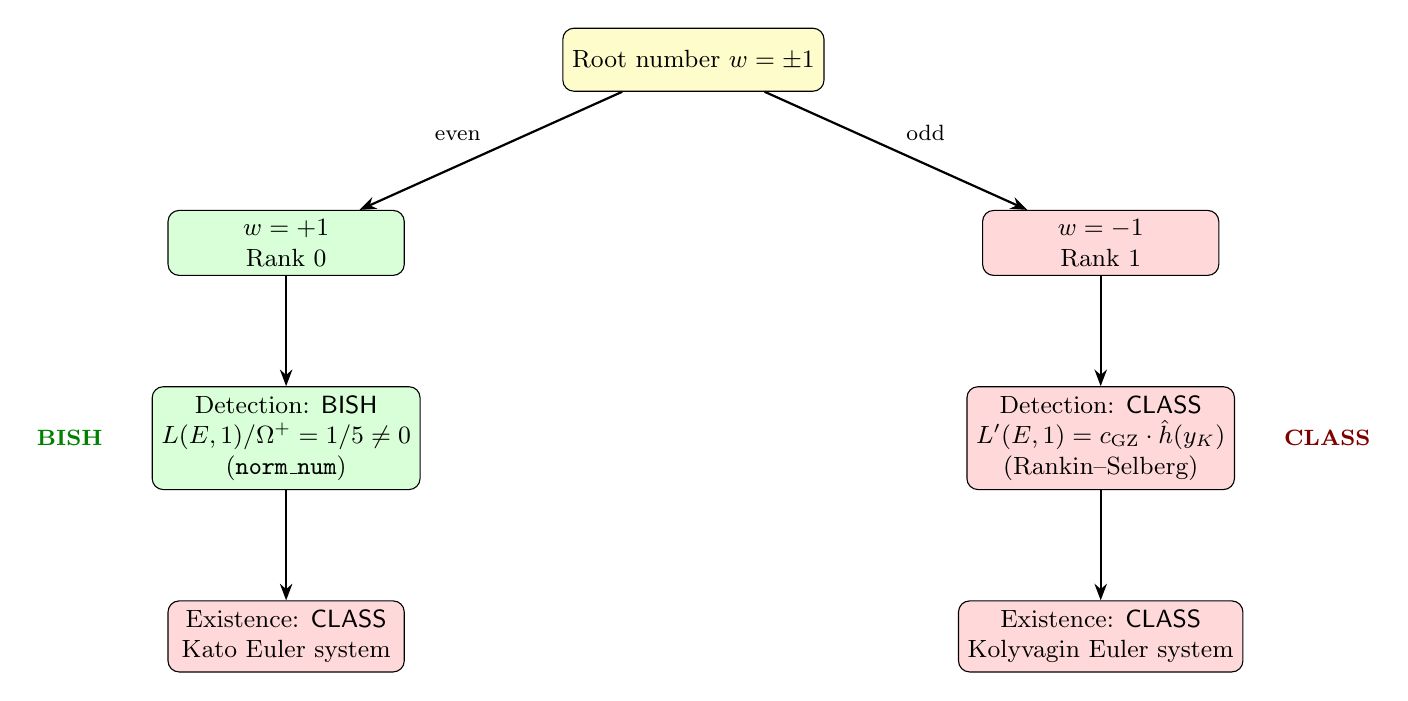
\begin{tikzpicture}[
  node distance=1.4cm and 3cm,
  bishbox/.style={draw, rounded corners, fill=green!15, minimum width=3cm, minimum height=0.8cm, align=center, font=\small},
  classbox/.style={draw, rounded corners, fill=red!15, minimum width=3cm, minimum height=0.8cm, align=center, font=\small},
  rootbox/.style={draw, rounded corners, fill=yellow!20, minimum width=3cm, minimum height=0.8cm, align=center, font=\small},
  arr/.style={-{Stealth[length=6pt]}, thick}
]

% Root
\node[rootbox] (root) {Root number $w = \pm 1$};

% Branches
\node[bishbox, below left=1.5cm and 2cm of root] (r0) {$w = +1$\\Rank 0};
\node[classbox, below right=1.5cm and 2cm of root] (r1) {$w = -1$\\Rank 1};

% Detection
\node[bishbox, below=of r0] (det0) {Detection: $\BISH$\\$L(E,1)/\Omega^+ = 1/5 \neq 0$\\(\texttt{norm\_num})};
\node[classbox, below=of r1] (det1) {Detection: $\CLASS$\\$L'(E,1) = c_{\mathrm{GZ}} \cdot \hhat(y_K)$\\(Rankin--Selberg)};

% Existence
\node[classbox, below=of det0] (ex0) {Existence: $\CLASS$\\Kato Euler system};
\node[classbox, below=of det1] (ex1) {Existence: $\CLASS$\\Kolyvagin Euler system};

% Arrows
\draw[arr] (root) -- node[above left, font=\footnotesize] {even} (r0);
\draw[arr] (root) -- node[above right, font=\footnotesize] {odd} (r1);
\draw[arr] (r0) -- (det0);
\draw[arr] (r1) -- (det1);
\draw[arr] (det0) -- (ex0);
\draw[arr] (det1) -- (ex1);

% Labels
\node[left=0.5cm of det0, font=\footnotesize, text=green!50!black] {\textbf{BISH}};
\node[right=0.5cm of det1, font=\footnotesize, text=red!50!black] {\textbf{CLASS}};

\end{tikzpicture}
\caption{The root number bifurcation. Detection is $\BISH$ for $w = +1$ and $\CLASS$ for $w = -1$. Existence is $\CLASS$ regardless.}
\label{fig:bifurcation}
\end{figure}


% ============================================================
\section{Discussion}
\label{sec:discussion}

\subsection{The de-omniscientising descent}

The root number bifurcation is a new instance of the de-omniscientising descent pattern of the series. The functional equation, a transcendental identity relating $L(E,s)$ at $s$ and $2-s$, has an algebraic consequence when $w = +1$: the modular symbol $L(E,1)/\Omega^+$ is nonzero and rational. This algebraic shadow is constructively accessible ($\BISH$), while the transcendental identity itself is $\CLASS$ (it requires analytic continuation to define $\Lambda(E,s)$ globally). The descent: from $\CLASS$ (analytic continuation) to $\BISH$ (modular symbol computation), mediated by the root number.

\subsection{Comparison with the Hodge bifurcation}

Paper~89 \cite{paper89} established the palindromic bifurcation in the Hodge campaign: when the characteristic polynomial of the genus-4 automorphism is palindromic ($a = c$), the Kani--Rosen splitting gives an unconditional Hodge class ($\BISH$ detection via Weyl's theorem). When $a \neq c$, Kani--Rosen fails and detection requires the Variational Hodge Conjecture ($\CLASS$).

The parallel is exact:
\begin{center}
\begin{tabular}{lll}
\toprule
& \textbf{BSD bifurcation} & \textbf{Hodge bifurcation} \\
\midrule
Invariant & Root number $w$ & Palindromic obstruction $a - c$ \\
$\BISH$ case & $w = +1$: modular symbol & $a = c$: Kani--Rosen \\
$\CLASS$ case & $w = -1$: Gross--Zagier & $a \neq c$: VHC \\
\bottomrule
\end{tabular}
\end{center}

In both cases, a \emph{computable algebraic invariant} ($w$, $a - c$) determines whether the detection mechanism stays within $\BISH$ or requires a transcendental input ($\CLASS$). This suggests a general principle: \emph{the CRM cost of arithmetic detection is controlled by computable symmetry invariants}.

\subsection{The descent excision}

Theorem~C shows that rank bounding can be separated from $\Sha$ finiteness. The 2-descent gives $\rk \leq 1$ for $\texttt{37a1}$ without Kolyvagin, at the cost of not proving $\Sha$ finiteness. This is a \emph{partial excision}: the $\CLASS$ content of the rank bound is removed, while the $\CLASS$ content of $\Sha$ finiteness remains.

For higher-rank curves ($\rk \geq 2$), the 2-descent becomes less effective (the 2-Selmer rank may exceed the true rank by the 2-rank of $\Sha$), and Kolyvagin's method is unavailable (it requires analytic rank $\leq 1$). The descent excision may thus be specific to the rank-1 case.

\subsection{Open questions}

\begin{enumerate}[nosep]
\item \textbf{Higher rank.} For rank~$\geq 2$, BSD is open. Does the root number bifurcation extend? For even analytic rank $r \geq 2$, $L^{(r)}(E,1)/r!$ might be computed by higher-order modular symbols ($\BISH$?), but this is speculative.
\item \textbf{Non-CM curves at rank 0.} Is there a rank-0 curve where the modular symbol computation requires more than \texttt{norm\_num}? For large conductor, the Hecke table is larger, but the detection mechanism (modular symbol $\neq 0$) remains $\BISH$ in principle.
\item \textbf{The Kato--Kolyvagin interface.} Can the $\CLASS$ content of Kato's Euler system (rank~0) be directly compared to Kolyvagin's (rank~1)? Both use Euler systems, but Kato's is algebraic $K$-theory while Kolyvagin's is Heegner points. A CRM comparison of the two $\CLASS$ shells is a natural follow-up.
\end{enumerate}


% ============================================================
\section{Conclusion}
\label{sec:conclusion}

This paper establishes the root number bifurcation for the CRM cost of BSD detection: $w = +1$ gives $\BISH$ (modular symbol), $w = -1$ gives $\CLASS$ (Gross--Zagier). The bifurcation is verified formally in Lean~4 (1{,}033~lines, 86~theorems, 0~\texttt{sorry}) with exceptionally clean axiom separation---the headline Theorem~B has zero axioms. The rank-0 audit ($10$~$\BISH$ + $3$~$\CLASS = 77\%$) improves on the rank-1 audit ($15$~$\BISH$ + $6$~$\CLASS = 71\%$) by eliminating the Gross--Zagier detection node. The descent excision (Theorem~C) shows that rank bounding is $\BISH$ via 2-descent, with $\Sha$ finiteness as the irreducible $\CLASS$ residue. The universal detection/existence table (Theorem~D) confirms, across four independent campaigns, that existence is universally $\CLASS$ and detection is $\BISH$ except when blocked by a computable invariant.


% ============================================================
\section*{Acknowledgments}

This paper was prepared with AI assistance (Anthropic Claude) for Lean~4 formalization and LaTeX composition. The mathematical content---CRM classification, root number bifurcation, descent excision---is due to the program's ongoing analysis, not to AI mathematical reasoning. Hecke eigenvalue and BSD data from Cremona's tables \cite{cremona} and the LMFDB \cite{lmfdb}. The Lean~4 formalization uses the Mathlib library \cite{mathlib4}; we thank the Mathlib contributors. This paper follows the CRM Series Format Guide \cite{format-guide}.

The author is an interventional cardiologist, not a domain expert in the mathematical areas treated here; all results should be considered preliminary and verified independently.


% ============================================================
\begin{thebibliography}{30}

\bibitem{bcdt}
C.~Breuil, B.~Conrad, F.~Diamond, R.~Taylor,
On the modularity of elliptic curves over~$\Q$: wild 3-adic exercises,
\emph{J.\ Amer.\ Math.\ Soc.}\ \textbf{14} (2001), 843--939.

\bibitem{bridges-richman}
D.~Bridges, F.~Richman,
\emph{Varieties of Constructive Mathematics},
London Math.\ Soc.\ Lecture Note Ser.\ \textbf{97}, Cambridge Univ.\ Press, 1987.

\bibitem{cassels-descent}
J.W.S.~Cassels,
Arithmetic on curves of genus~1.\ IV.\ Proof of the Hauptvermutung,
\emph{J.\ Reine Angew.\ Math.}\ \textbf{211} (1962), 95--112.

\bibitem{cremona}
J.E.~Cremona,
\emph{Algorithms for Modular Elliptic Curves}, 2nd ed.,
Cambridge Univ.\ Press, 1997.

\bibitem{format-guide}
P.C.K.~Lee,
CRM Series Format Guide,

\bibitem{gross-zagier}
B.H.~Gross, D.B.~Zagier,
Heegner points and derivatives of $L$-series,
\emph{Invent.\ Math.}\ \textbf{84} (1986), 225--320.

\bibitem{kato}
K.~Kato,
$p$-adic Hodge theory and values of zeta functions of modular forms,
\emph{Ast\'erisque}\ \textbf{295} (2004), 117--290.

\bibitem{kolyvagin1988}
V.A.~Kolyvagin,
Finiteness of $E(\Q)$ and $\Sha(E,\Q)$ for a subclass of Weil curves,
\emph{Izv.\ Akad.\ Nauk SSSR Ser.\ Mat.}\ \textbf{52} (1988), 522--540.

\bibitem{kolyvagin1990}
V.A.~Kolyvagin,
Euler systems,
in: \emph{The Grothendieck Festschrift}, Vol.~II, Progr.\ Math.\ \textbf{87}, Birkh\"auser, 1990, pp.~435--483.

\bibitem{lmfdb}
The LMFDB Collaboration,
\emph{The L-functions and Modular Forms Database},
\url{https://www.lmfdb.org}, 2024.

\bibitem{manin}
Ju.I.~Manin,
Parabolic points and zeta functions of modular curves,
\emph{Izv.\ Akad.\ Nauk SSSR Ser.\ Mat.}\ \textbf{36} (1972), 19--66.

\bibitem{mathlib4}
The Mathlib Community,
\emph{Mathlib4: Mathematical Library for Lean 4},
Zenodo, 2024. \texttt{DOI: 10.5281/zenodo.8127963}.

\bibitem{mazur}
B.~Mazur,
Modular curves and the Eisenstein ideal,
\emph{Inst.\ Hautes \'Etudes Sci.\ Publ.\ Math.}\ \textbf{47} (1977), 33--186.

\bibitem{paper1}
P.C.K.~Lee,
The logical cost of Zorn's lemma (Paper~1, CRM Series),
Zenodo, 2025. \texttt{DOI: 10.5281/zenodo.15086879}.

\bibitem{paper40}
P.C.K.~Lee,
The physics ceiling (Paper~40, CRM Series),
Zenodo, 2025. \texttt{DOI: 10.5281/zenodo.15278001}.

\bibitem{paper48}
P.C.K.~Lee,
The logical cost of BSD: LPO and the Archimedean escape (Paper~48, CRM Series),
Zenodo, 2025. \texttt{DOI: 10.5281/zenodo.18683400}.

\bibitem{paper51}
P.C.K.~Lee,
The Archimedean rescue for BSD rank one (Paper~51, CRM Series),
Zenodo, 2025. \texttt{DOI: 10.5281/zenodo.18732168}.

\bibitem{paper80}
P.C.K.~Lee,
Algebraic Gauss--Manin via Griffiths pole reduction: a CRMLint Squeeze (Paper~80, CRM Series),
Zenodo, 2026. \texttt{DOI: 10.5281/zenodo.18791985}.

\bibitem{paper89}
P.C.K.~Lee,
Absolute Hodge classes for the universal hyperelliptic Weil locus: a CRMLint Squeeze (Paper~89, CRM Series),
Zenodo, 2026. \texttt{DOI: 10.5281/zenodo.18809909}.

\bibitem{paper90}
P.C.K.~Lee,
The Squeeze is a microscope: automated constructivization from CRMLint to the Hodge horizon (Paper~90, CRM Series),
Zenodo, 2026. \texttt{DOI: 10.5281/zenodo.18809911}.

\bibitem{paper94}
P.C.K.~Lee,
The Griffiths group of the mirror quintic: a CRMLint Squeeze (Paper~94, CRM Series),
Zenodo, 2026. \texttt{DOI: 10.5281/zenodo.18820969}.

\bibitem{paper95}
P.C.K.~Lee,
The BSD Squeeze: CRMLint decomposition of the Gross--Zagier--Kolyvagin proof (Paper~95, CRM Series),
Zenodo, 2026. \texttt{DOI: 10.5281/zenodo.18821019}.

\bibitem{silverman-aec}
J.H.~Silverman,
\emph{The Arithmetic of Elliptic Curves}, 2nd ed.,
Grad.\ Texts in Math.\ \textbf{106}, Springer, 2009.

\bibitem{taylor-wiles}
R.~Taylor, A.~Wiles,
Ring-theoretic properties of certain Hecke algebras,
\emph{Ann.\ of Math.}\ \textbf{141} (1995), 553--572.

\bibitem{wiles}
A.~Wiles,
Modular elliptic curves and Fermat's Last Theorem,
\emph{Ann.\ of Math.}\ \textbf{141} (1995), 443--551.

\end{thebibliography}

\end{document}
